Ein wesentlicher Teil dieser Arbeit besteht in der softwareseitigen Realisierung
der Laserstabilisierung und Experimentsteuerung. In diesem Kapitel sollen daher
alle Softwarekomponenten genauer betrachtet werden. Abschnitt
\ref{sec:datenerfassung_der_laser} wird beschrieben, wie die Informationen
der Laserfrequenzen aus der Counterkarte ausgelesen, im
Mikrocontroller \textit{Arduino} aufbereitet und anschließend am PC ausgewertet
werden. In Abschn. \ref{sec:stabilisierung_frequenzverstimmungs-strategie} wird die Regelung
der Laserfrequenz und der damit verbundenen Strategie der Frequenzverstimmung
erklärt. Abschnitt \ref{sec:linearisierung_iscan} beschäftigt sich mit der
Linearisierung der \textit{iScans} und dem Neuschreiben der LUT. Die
Benutzerschnittstelle zur Experimentsteuerung soll in Abschn.
\ref{sec:experimentsteuerung} behandelt werden. In Abschn. \ref{sec:sonstiges}
werden weitere Funktionen kurz angerissen. Da die Software am PC in
Labview entwickelt wurde und somit der Code nur sehr platzverschwendend
dargestellt werden kann, wird die Beschreibung ausschließlich über
Ablaufdiagramme und Bildschirmfotos der Benutzeroberfläche geschehen. Der
Quellcode des Labview-Programms kann am Kontrollrechner selbst eingesehen
werden. Programme in Labview werden im Folgenden \textit{Virtuelles
Instrument} (VI) bzw. SubVI (Unterprogramm) genannt.

\section{Datenerfassung der Laser}\label{sec:datenerfassung_der_laser}
Die Informationen der Laser durchlaufen mehrere Stufen der Signal- und
Datenverarbeitung, bis eine quantitative Aussage über das Frequenzverhalten
gemacht werden und eine Regelroutine anlaufen kann. Der erste Teil der
Datenaufbereitung verläuft rein elektronisch, bis die Counterwerte binär in
den Counterregistern abrufbereit vorliegen, wie bereits in Abschn.
\ref{sec:elektronik_laserkontrolle} ausführlich erklärt wurde. An dieser Stelle
setzt nun die softwareseitige Weiterverarbeitung an. Im Folgenden wird sich
wieder exemplarisch nur auf einen Diodenlaser und den Referenzlaser bezogen.
Für alle anderen Laser gilt der identische Ablauf.

\subsection{Datenaufbereitung}\label{subsec:datenaufbereitung}
Zunächst werden die Counterwerte mithilfe des Mikrocontrollers \textit{Arduino}
ausgelesen und verarbeitet. Das komplette Ablaufdiagramm der Software des
\textit{Arduinos} ist in Abb. \ref{fig:ablaufdiagramm_arduino_laser} in auf die
wesentlichen Teile gekürzter Form zu sehen. Der komplette Quellcode hierfür
wurde in der Programmiersprache C geschrieben und ist im Anhang
\ref{anh:kap:quelltext_arduino_laserinformationsverarbeitung} zu finden.
\begin{figure}[hp]
 	\centering
 	\fbox{\parbox{\dimexpr \linewidth - 2\fboxrule - 2\fboxsep}{
 	\centering
	    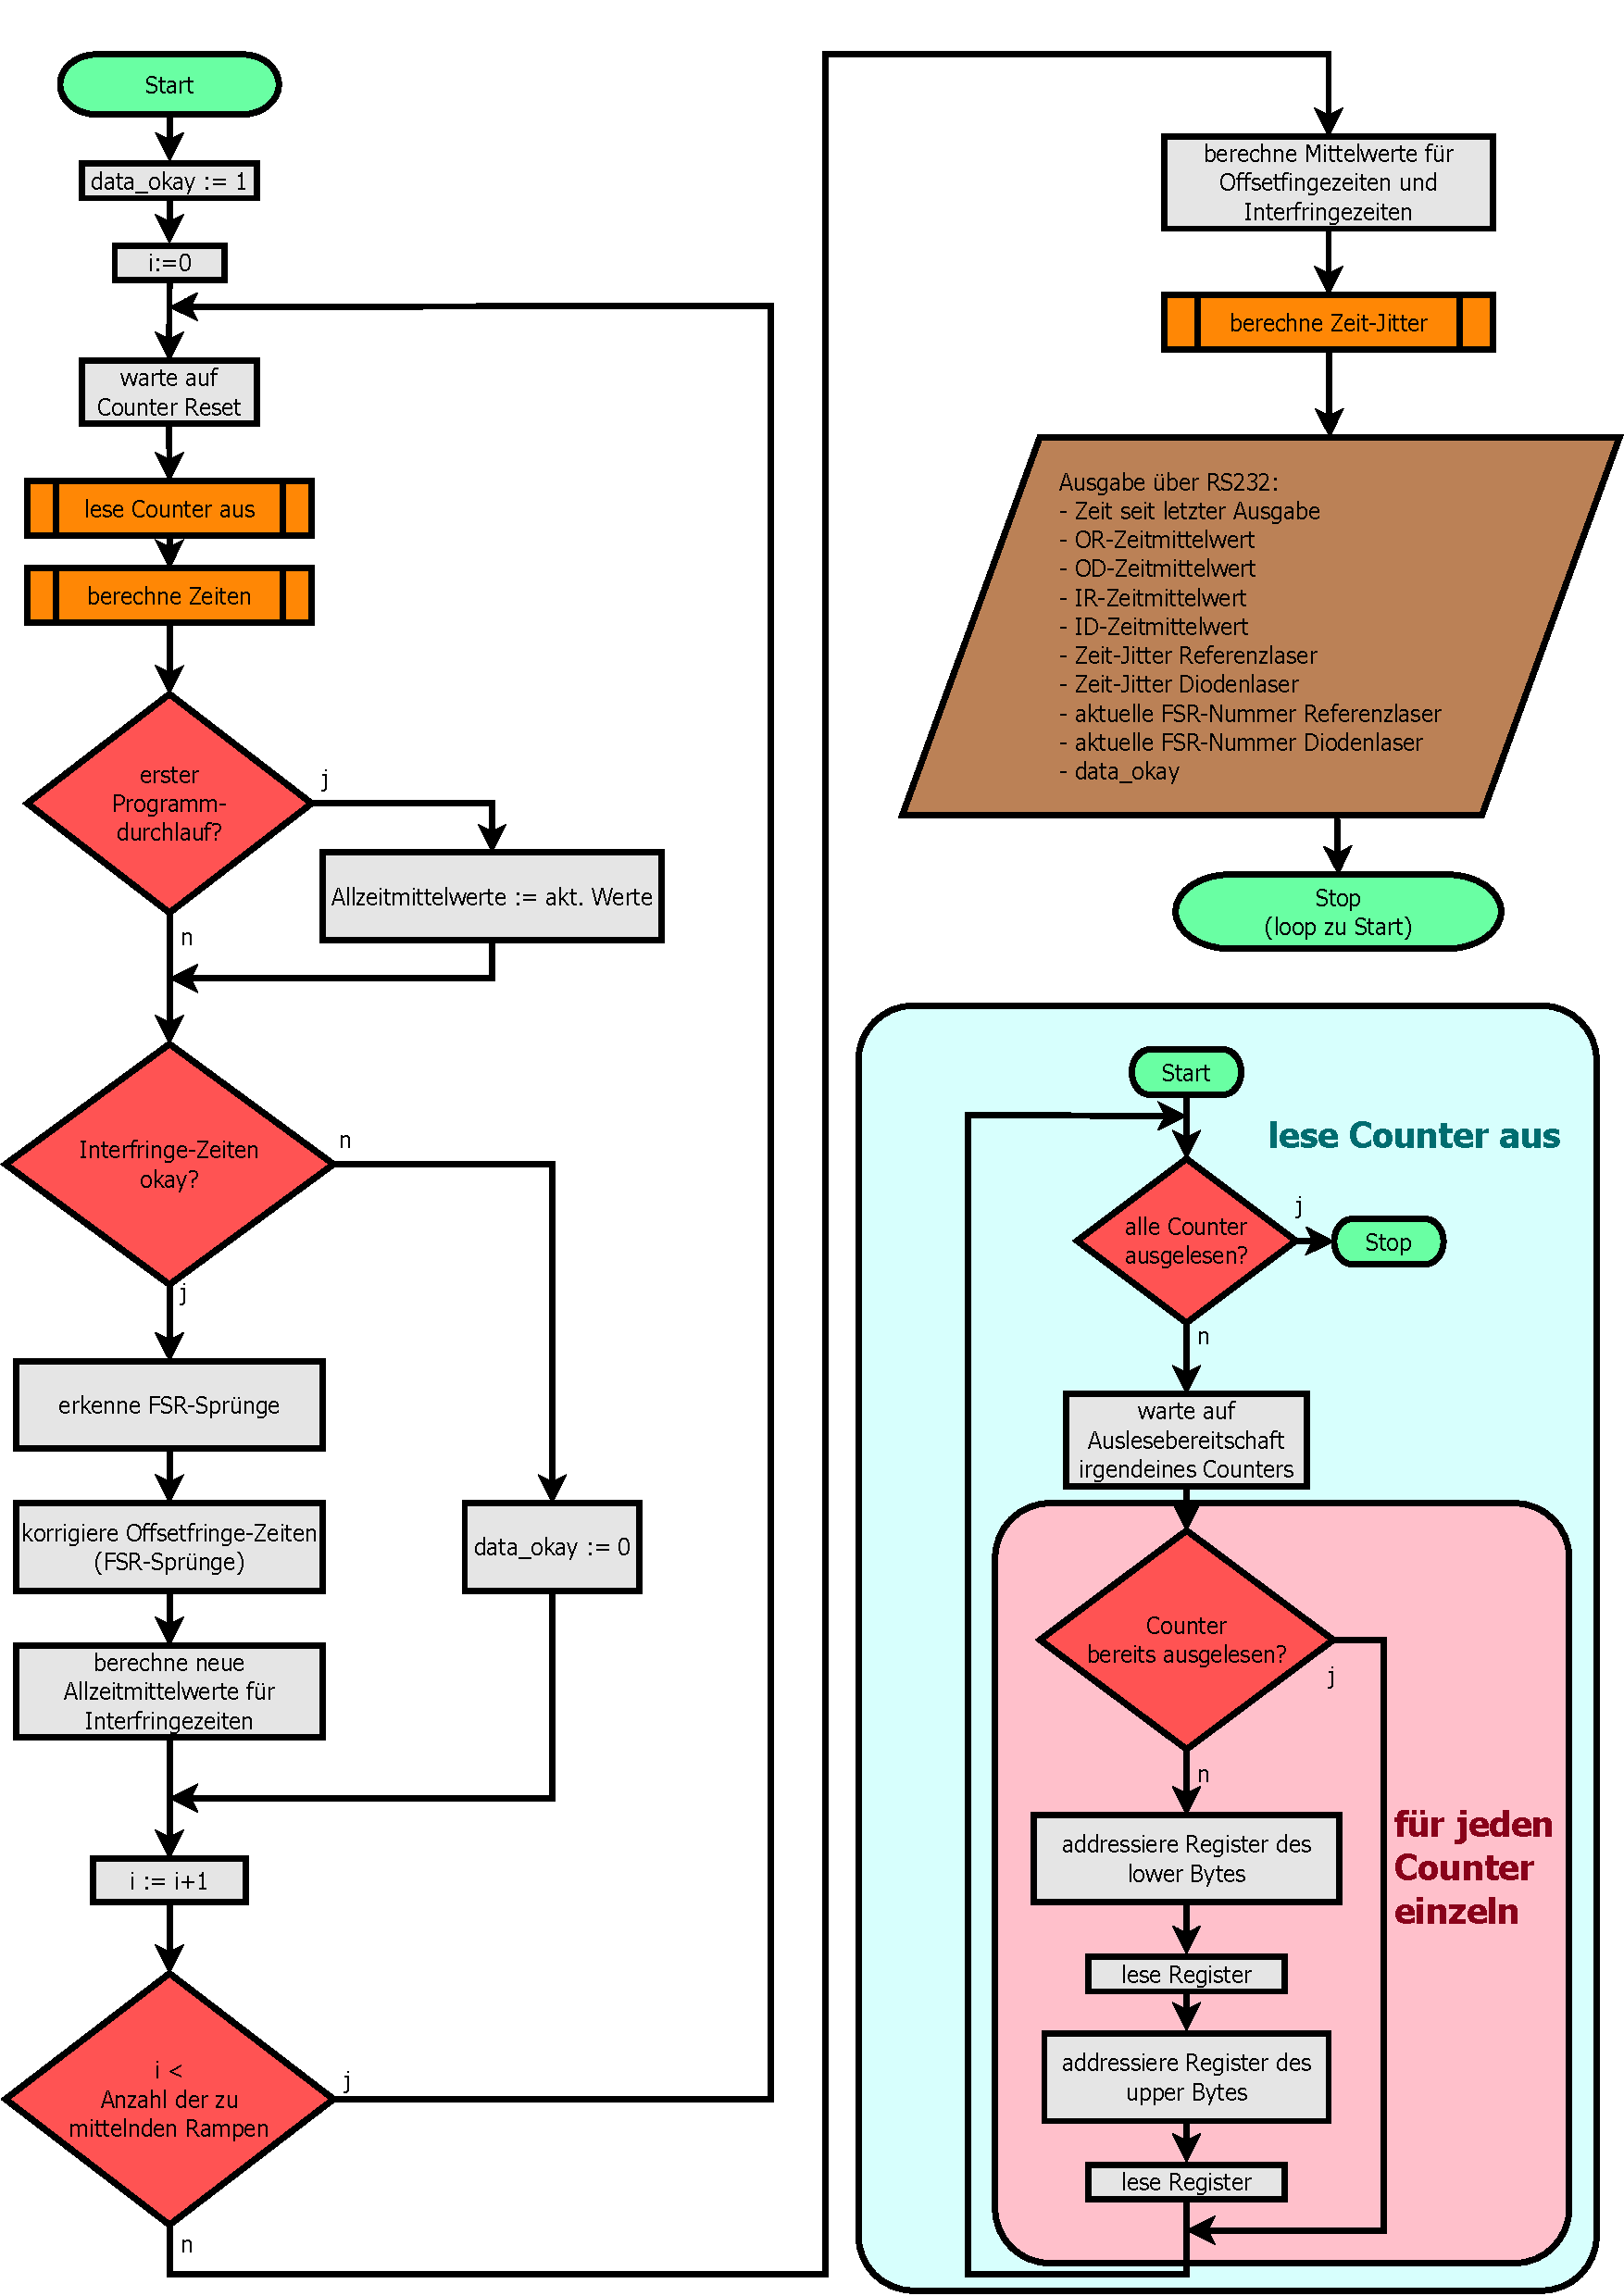
\includegraphics[width=\textwidth-0.5cm]{gfx/ablaufdiagramm_arduino_laser}
	    }}
	\caption[Laserdatenaufbereitung -
	Ablaufdiagramm]{Ablaufdiagramm der
	Laserdatenaufbereitung}\label{fig:ablaufdiagramm_arduino_laser}
\end{figure}
Der \textit{Arduino} verfügt über 54 digitale Ein- und Ausgänge, welche der
Kommunikation mit der Counterkarte dienen. HIGH ($5\,$V) bzw. LOW ($0\,$V) wird
als 1 bzw. 0 oder TRUE bzw. FALSE interpretiert. Das Programm besteht aus
einem
\textit{Setup}, in dem initialisierende Routinen wie beispielsweise die
Pinbelegung abgearbeitet werden, und einer \textit{Endlosschleife} (\textit{Start}$\rightarrow$\textit{Programm}$\rightarrow$\textit{Stop}$\rightarrow$\textit{Start}$\rightarrow$\ldots),
über die die stetige Überwachung der Laser abgewickelt wird. Die Aufgaben des
Programms sind
\begin{itemize}
	\item Counter auslesen
	\item reale Zeiten berechnen
	\item unplausible Zeiten ignorieren
	\item FSR-Sprünge erkennen und Zeiten korrigieren
	\item Mittelwerte der Zeiten bilden.
	\item Laser-Jitter berechnen.
\end{itemize}
All dies muss innerhalb eines Rampenzyklusses (also innerhalb von maximal
$17\,$ms) geschehen, damit keine Information verloren geht. Im schlimmsten Fall
bleibt dem Mikrocontroller für die Berechnungen nach dem Auslesen der Counter
nur ca. $2\,$ms (fallende Rampe). Aus diesem Grund wurde das Programm möglichst
performand programmiert.\par Es wird immer eine bestimmte Anzahl von Rampenzyklen zusammengefasst und Zeitmittelwerte für die Offset- und Interfringezeiten beider Laser ($t_{OR,i}$,
$t_{OD,i}$, $t_{IR,i}$ und $t_{ID,i}$) berechnet. Weiterhin wird aus der
Standardabweichung der Offsetfringezeiten der Jitter
\begin{equation}\label{eq:jitter_zeit}
	\Delta
	t_O=\sqrt{\frac{1}{n-1}\cdot\sum\limits_{i=1}^{n}\left(t_{O,i}-\overline{t}_O\right)^2}
\end{equation}
des jeweiligen Lasers über die Anzahl der zu mittelnden Rampenzyklen
ermittelt.\par
Eine Iteration beginnt - wenn nötig - mit dem Warten bis alle
Counter zurückgesetzt wurden, indem geprüft wird, ob alle Status-Bits LOW sind, was irgendwann während der fallenden Rampe geschieht.
Anschließend werden die Counter ausgelesen. Dabei wird in einer Schleife zu
Beginn geprüft, ob bereits alle Counter ausgelesen worden sind. Wenn dies nicht
der Fall ist, wird über die Status-Bits auf die Bereitschaft irgendeines
Counters gewartet und im Falle der Bereitschaft geprüft, ob der Counter schon
ausgelesen worden ist. Wurden die Werte noch nicht ausgelesen, werden upper und
lower Byte nacheinander adressiert und ausgelesen.\par
Aus den erhaltenen 16-Bit-Werten werden nun über die fest einprogrammierte
Taktrate die wirklichen Zeiten berechnet. Während der gesamten Laufzeit des
Programms werden nach jeder Iteration
Allzeitmittelwerte für die Interfringezeiten erneuert. Zu Beginn des Programms werden diese mit den ersten
Zeiten initialisiert. Mithilfe der Allzeitmittelwerte wird geprüft, ob die
aktuellen Interfringezeiten valide sind. Es kann insbesondere bei schnellen
Frequenzverstimmungen vorkommen, dass während einer Rampe der Interfringe aus
dem aktuellen FSR hinausläuft, noch bevor der Counter gestoppt wurde und
somit eine falsche Zeit gemessen wird. Um diese Fälle und andere Fehlmessungen
auszusondern, wird geprüft, ob die gemessene Interfringezeit stark vom
Allzeitmittelwert abweicht. Bei offensichtlich falscher Messung wird die
momentane Iteration abgebrochen und für die spätere Ausgabe ein
Validitätsvariable auf 0 gesetzt, damit bei der Weiterverarbeitung am PC
entschieden werden kann, ob die Daten genutzt werden möchten oder nicht.\par
Sind die Zeiten valide, kann herausgefunden werden, ob die Laserfrequenz des
Diodenlaser in einen benachbarten FSR des FPIs gelaufen ist. Dabei wird
überprüft, ob sich die Zeit des Offsetfringes relativ gemessen zur
Offsetfringezeit des Referenzlasers gegenüber der Zeit der vorherigen Rampe um mehr als die Hälfte der Interfringezeit verändert hat. Folgendes kann auftreten:
\begin{subequations}\label{eq:FSR-sprung}
	\begin{equation}\label{eq:FSR-sprung_links}
		(t_{OD,akt.}-t_{OR,akt.})-(t_{OD,alt}-t_{OR,alt})>\nicefrac{1}{2}\cdot
t_{ID,akt}
	\end{equation}
	\begin{equation}\label{eq:FSR-sprung_rechts}
		(t_{OD,akt.}-t_{OR,akt.})-(t_{OD,alt}-t_{OR,alt})<-\nicefrac{1}{2}\cdot
t_{ID,akt}\,.
	\end{equation}
\end{subequations}
Gilt \eqref{eq:FSR-sprung_links}, so wird vermutet, dass der Laser in den links
benachbarten FSR gedriftet ist. Im Falle von \eqref{eq:FSR-sprung_rechts} ist
der Laser vermutlich in den rechts benachbarten FSR gedriftet. In
beiden Fällen wird eine FSR-Nummer-Variable erniedrigt bzw. erhöht, um später am
PC die FSR-Sprünge zählen zu können. Die Detektion kann natürlich wie schon
erwähnt nur funktionieren, wenn die Frequenz deutlich langsamer als
$\nicefrac{\text{FSR}}{2}$ pro Rampenzyklus verstimmt wird. Damit auch bei
FSR-Sprüngen die Zeiten zur Mittelung beitragen können, werden diese anschleißend durch subtrahieren bzw. addieren der Interfringezeit korrigiert.\par
Für den Referenzlaser ist ein FSR-Sprung aufgrund seiner absoluten Stabilität
bis auf wenige MHz praktisch unmöglich, sofern des Offset der Rampe so
eingestellt ist, dass der erste Fringe ca.
$\nicefrac{\text{FSR}}{2}$ nach Start der Rampe auftaucht. Somit bleibt die
Laserfrequenz mit aller Sicherheit immer in demselben FSR des FPIs. Es
kommt jedoch vor, dass die Rampe oder das FPI einem Drift unterliegen
und der Referenzlaser scheinbar in einen benachbarten FSR driftet.
Analog wie beim Diodenlaser wird auch hier der scheinbare FSR-Sprung
detektiert. In diesem Fall wird aber lediglich die Offsetfringezeit wie beim
Diodenlaser korrigiert. Die Zählvariable für den scheinbaren FSR-Sprung
wird nur noch zu Debugzwecken aufbewahrt. Logischerweise können
gleichzeitige FSR-Sprünge beider Laser so nicht erkannt werden. In diesem
sehr unwahrscheinlichen Fall käme es zu Fehlberechnungen der Relativfrequenz.
Um dennoch sicher zu sein, sollte deshalb regelmäßig auf die Lage des ersten
He:Ne-Fringes geachtet und ggf. das Offset der Rampe nachkorrigiert werden.\par
Wurden genügend Rampen durchlaufen, können die aktuellen Mittelwerte aller
Zeiten und die Standardabweichung der Offsetfringezeiten berechnet und mit allen
anderen nötigen Werten über eine RS232-Schnittstelle an den PC gesandt werden
(brauner Kasten in Abb.
\ref{fig:ablaufdiagramm_arduino_laser}). Der String der versandt wird, beginnt
mit \lstinline|"*begin*"| und endet mit \lstinline|"*end*"|, damit später
sichergestellt werden kann, wo die Daten anfangen und aufhören. Die Werte sind
untereinander durch Leerzeichen getrennt.

\subsection{Datenbereitstellung am PC}\label{subsec:datenbereitstellung}
Die Daten eines jeden Lasers kommen wie oben erwähnt als String in Zeitabständen
eines Vielfachen der Rampendauer am PC an. Damit es zu keinem Pufferstau an
der seriellen Schnittstelle des PCs kommt, werden die aktuellen Strings direkt
nach Abschneiden von \lstinline|"*begin*"| und \lstinline|"*end*"| durch das
SubVI \lstinline|arduino_laser_read.vi| in globale Variablen geschrieben.
Parallel wird jeweils eine boolsche Variable gesetzt, die angibt, dass die Laserinformationen aktuell sind. Wird ein String aus einer der
globalen Variablen gelesen, wird die boolsche Variable zurückgesetzt und die
Laserinformationen werden als nicht mehr aktuell gewertet. Aktualität fordernde
Lesezugriffe auf die Daten warten, bis die Variable wieder gesetzt wurde. Die
aktuellen Zeiten können nun separat über das SubVI
\lstinline|get_laser_times.vi| nach Angabe der Lasernummer abgeholt werden. Das SubVI \lstinline|delta_time2delta_frequency.vi| berechnet nach Gl. \eqref{eq:FPI_frequenzdrift_03} aus den Zeiten die
Relativfrequenzen. Das SubVI \lstinline|laser-control.vi|, das in Abschn.
\ref{sec:stabilisierung_frequenzverstimmungs-strategie} näher betrachtet wird, hat neben der Regelung und Frequenzverstimmtung auf die Sollfrequenz auch die Aufgabe
Monitoringdaten an die Benutzeroberfläche der Laserkontrolle (Abb.
\ref{fig:benutzeroberflaeche_laserkontrolle}) weiterzugeben. Zu den
Monitoringdaten gehören Jitter des Lasers, Ist-Relativfrequenz und Abweichung
zur Soll-Relativfrequenz, wobei die detektierten FSR-Sprünge mit einbezogen
werden müssen. Die Referenzfrequenz ist beim Start des Programms oder beim
Drücken des Buttons \lstinline|assign| die derzeit aktuelle Laserfrequenz.
\begin{figure}[h]
 	\centering
 	\fbox{\parbox{\dimexpr \linewidth - 2\fboxrule - 2\fboxsep}{
 	\centering
	    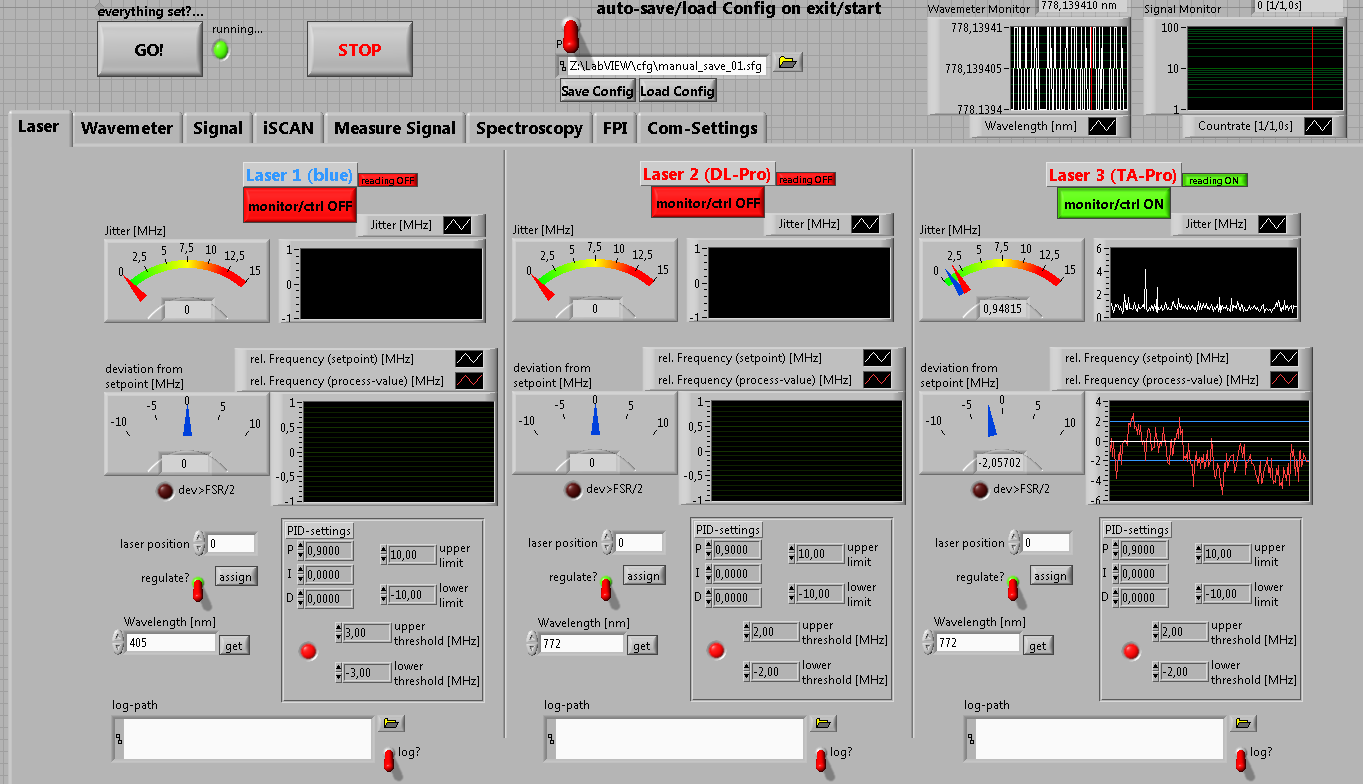
\includegraphics[width=\textwidth-0.5cm]{gfx/benutzeroberflaeche_laserkontrolle}
	    }}
	\caption[Benutzeroberfläche -
	Laserkontrolle]{Benutzeroberfläche
	der Laserkontrolle}\label{fig:benutzeroberflaeche_laserkontrolle}
\end{figure}

\section{Stabilisierung/Frequenzverstimmungs-Strategie}\label{sec:stabilisierung_frequenzverstimmungs-strategie}
Frequenzverstimmung und gleichzeitige Regelung wird von der SubVI
\lstinline|laser-control.vi| verwaltet. Die Anforderungen sind möglichst
schnelles Anfahren der Sollfrequenz, egal, wie groß die Verstimmung ist, und
anschließendes Regeln. Alle im Folgenden verwendete Frequenzangaben sind
Relativfrequenzen zu einer zu Beginn festgelegten Nullfrequenz. Grundidee ist,
dass der Laser über das \textit{iScan} sehr schnell in den Bereich der
Sollfrequenz gefahren wird und anschließend mithilfe des FOLs nachgeregelt wird,
da ein direktes Anfahren mit dem \textit{iScan} aufgrund seiner Nichtliniearität unmöglich ist. In Kap. \ref{kap:charakterisierung} wird sich zeigen, dass der Fehler bei
alleiniger Verstimmung mit dem \textit{iScan} wenige bis mehr als $100\,$MHz sein kann.
Dies bedarf einer nicht-trivialen Strategie, die mithilfe von Abb.
\ref{fig:frequenzverstimmungs-strategie} und dem Ablaufdiagramm
\ref{fig:frequenzverstimmungs-strategie_ablaufdiagramm} veranschaulicht werden
soll.\par
\begin{figure}[h]
 	\centering
 	\fbox{\parbox{\dimexpr \linewidth - 2\fboxrule - 2\fboxsep}{
 	\centering
	    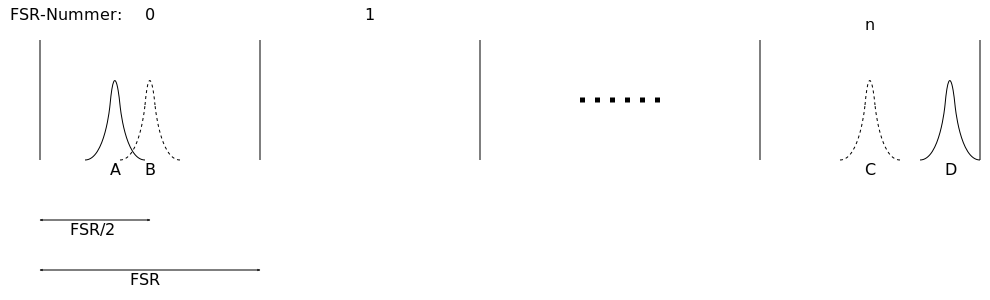
\includegraphics[width=\textwidth-0.5cm]{gfx/frequenzverstimmungs-strategie}
	    }}
	\caption[Frequenzverstimmungs-Strategie]{Frequenzverstimmungs-Strategie,
	Erklärung im Text.}\label{fig:frequenzverstimmungs-strategie}
\end{figure}
\begin{figure}[hp]
 	\centering
 	\fbox{\parbox{\dimexpr \linewidth - 2\fboxrule - 2\fboxsep}{
 	\centering
	    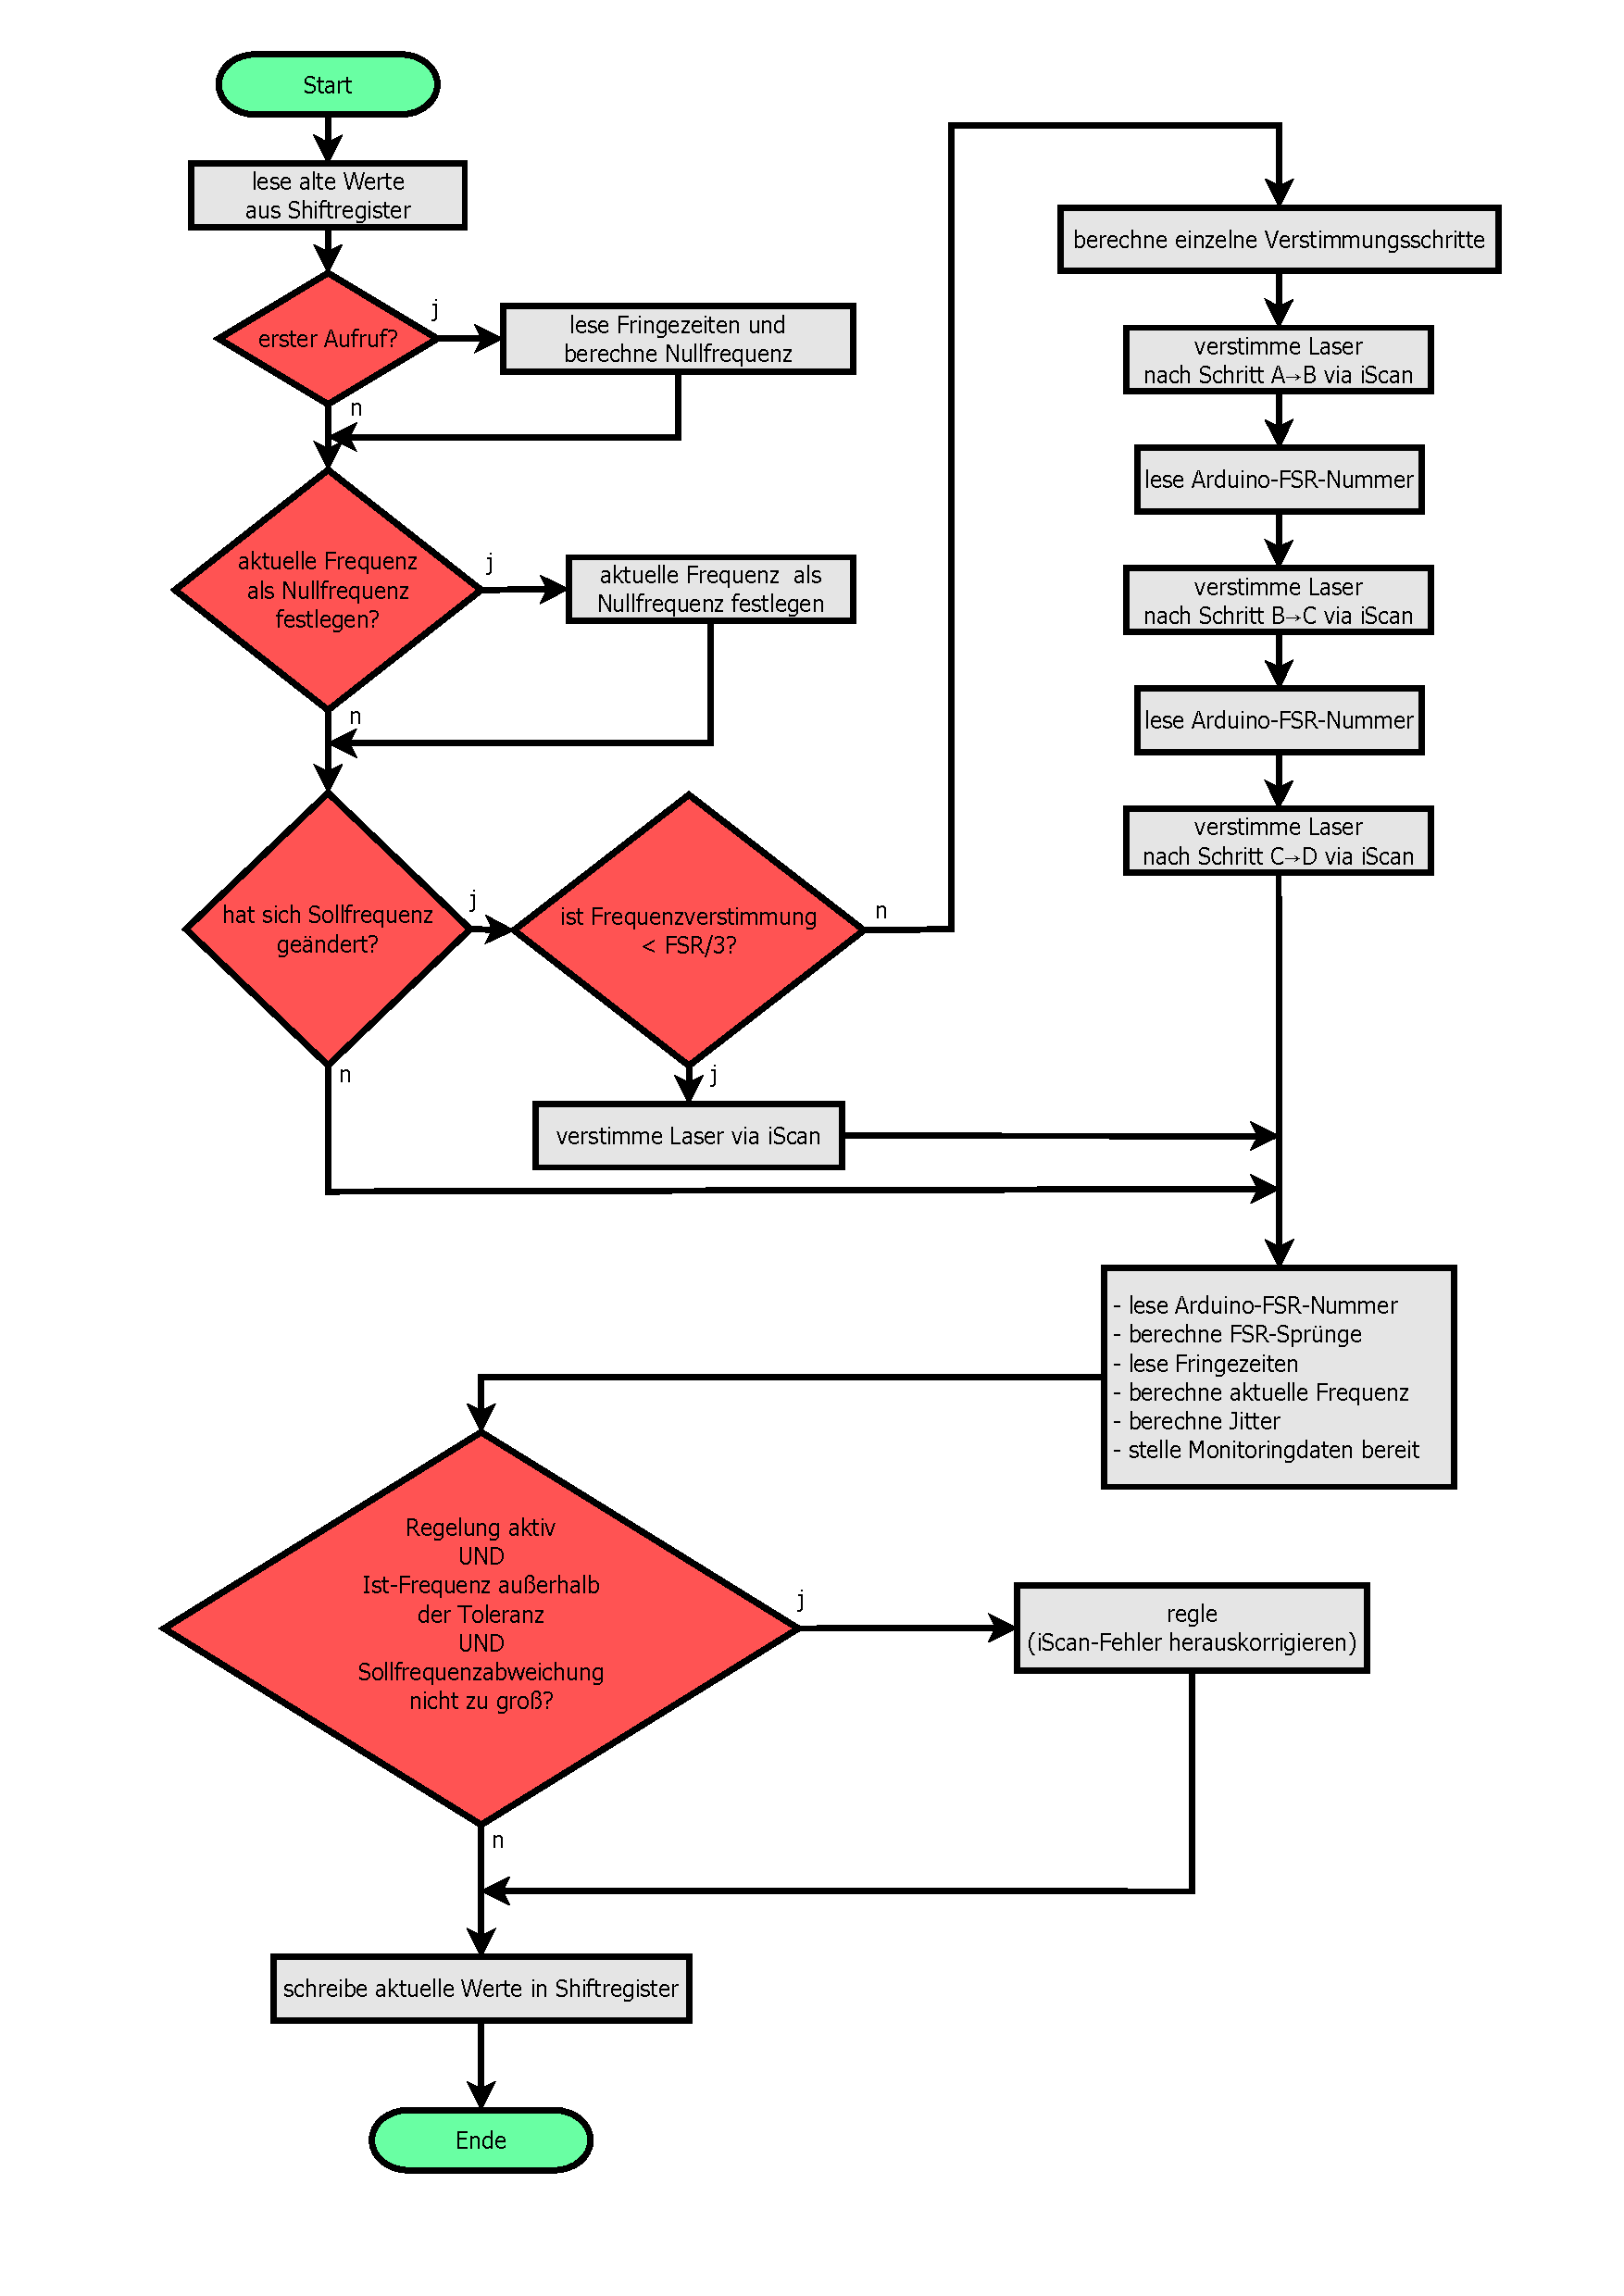
\includegraphics[width=\textwidth-0.5cm]{gfx/frequenzverstimmungs-strategie_ablaufdiagramm}
	    }}
	\caption[Frequenzverstimmungs-Strategie
	-
	Ablaufdiagramm]{Frequenzverstimmungs-Strategie
	Ablaufdiagramm}\label{fig:frequenzverstimmungs-strategie_ablaufdiagramm}
\end{figure}
Naiverweise könnte man die Strategie verfolgen, den zu verstimmenden
Frequenzwert in ein Vielfaches $n$ des FSRs und einen Rest aufzuteilen. Mit dem
\textit{iScan} würde man den Laser um $n\cdot\text{FSR}$ schnell verfahren,
die aktuelle FSR-Nummer $n_{Ard,1}$ vom \textit{Arduino} auslesen und anschließend
noch die Restfrequenz mit dem \textit{iScan} in drei gleich großen
Schritten\footnote{Der Rest des Verstimmungsvorgangs würde in drei Schritte
aufgeteilt, damit der Laser pro Schritte maximal um $\nicefrac{\text{FSR}}{3}$
pro Schritt verfahren würde.} verfahren. Zwischen jedem Einzelschritt würde
$17\,$ms gewartet werden, damit ein eventueller FSR-Sprung detektiert werden
kann.
Nach einem erneuten Abfragen der FSR-Nummer $n_{Ard,2}$ könnte man aus der zu
verstimmenden Frequenz $\Delta\nu$ die erreichte Frequenz über
\begin{equation}\label{eq:neue_frequenz_strategie_1}
	\begin{split}
		\nu_{Ist,nach} &=
		n_{Lab,nach}\cdot\text{FSR}+(\nu_{Offset,nach}-\nu_{Offset,vor})\\
		\text{mit}\quad
		n_{Lab,nach} &= n_{Lab,vor}+n+(n_{Ard,2}-n_{Ard,1})\\
		\text{und}\quad
		n &= \left\lfloor\frac{\Delta\nu}{\text{FSR}}\right\rfloor\,,
	\end{split}
\end{equation}
berechnen, wobei $n_{Lab,nach}$ bzw. $n_{Lab,vor}$ die von Labview
verwaltete FSR-Nummer und $\nu_{Offset,nach}$ bzw. $\nu_{Offset,vor}$ die
Frequenzposition des Lasers im FSR realtiv zum Referenzlaser nach bzw. vor der
Verstimmung sind. Das Nachkorrigieren des \textit{iScan}-Fehlers
$\nu_{Ist}-\nu_{Soll}$ würde dann das FOL übernehmen, das wie in Abschnitt
\ref{sec:iscan_und_fringe-offset-locking} erklärt auch für den Driftausgleich
zuständig ist.\par
Diese Strategie setzt aber eine wichtige und nie sicher gegebene Tatsache
vorraus: Bei dem ersten Frequenzverstimmungsschritt $n\cdot\text{FSR}$ geht man
immer davon aus, dass man im $n$-ten FSR des FPIs relativ zur Ausgangsposition
landet. Darauf muss man sich verlassen können, denn eine FSR-Sprung-Detektion
des \textit{Arduinos} ist hier aufgrund des schnellen Verstimmens nicht möglich
und wird schlicht ignoriert. Das Problem hieran ist nun, dass es durchaus vorkommen kann,
wegen dem \textit{iScan}-Fehler nicht im erwarteten FSR zu landet und somit am
Ende einen Fehler von $\pm\text{FSR}$ in der Frequenzberechnung zu erhalten.
Folgende Strategie kann dieses Problem zwar nicht komplett ausschließen, ist aber
wesentlich sicherer, sofern der maximale Verstimmungsfehler des \textit{iScans}
$<\nicefrac{\text{FSR}}{2}$, also ca. $150MHz$ ist.\par
Die Frequnenzverstimmungsmethode besteht aus drei Hauptschritten. Im ersten
Schritt ($A\rightarrow B$) wird der Laser auf eine Frequenz verstimmt, deren
Fringe sich in der Mitte des aktuellen FSRs befindet. Dieser Schritt erfolgt in
zwei gleich großen Teilschritten (maximal $\nicefrac{\text{FSR}}{4}$) mit je
anschließender Pause von $17\,$ms, um sicher FSR-Sprünge detektieren zu können.
Nach einer Abfrage der FSR-Nummer $n_{Ard,1}$ vom \textit{Arduino} folgen zweiter und dritter Schritt ($B\rightarrow C$ und $C\rightarrow D$) analog zur
vorherigen Überlegung (also ein ganzzahliges Vielfaches von FSR im zweiten
Schritt und der Rest im dritten Schritt). Der Fehler im Schritt $B\rightarrow C$
darf also maximal $\nicefrac{\text{FSR}}{2}$ sein, damit der erwartete FSR erreicht wird. Die Verstimmnungsfrequnenzen der einzelnen Schritte ergeben sich aus
\begin{equation}\label{eq:scan-strategie_schritte}
	\begin{split}
		\Delta\nu_{A\rightarrow B}&=\frac{\text{FSR}}{2}-\nu_{Offset,vor}\\
		\Delta\nu_{B\rightarrow
		C}&=\left\lfloor\frac{(\Delta\nu-\Delta\nu_{A\rightarrow
		B})}{\text{FSR}}\right\rfloor\cdot\text{FSR}\\
		\Delta\nu_{C\rightarrow D}&=(\Delta\nu-\Delta\nu_{A\rightarrow
		B})\mod\text{FSR}\,,
	\end{split}
\end{equation}
wobei $\Delta\nu$ die zu verstimmende Frequenz ist.
Die zeitliche Abfolge ist in Tab. \ref{tab:scan-strategie_abfolge} noch einmal
zusammengefasst.
\begin{table}
	%Summe der Breiten muss 0.91 mal \textwidth sein.
	\begin{tabular}{p{0.05\textwidth}p{0.86\textwidth}}
		\toprule
			Nr. & Beschreibung \\
		\midrule[1px]
		\hline
			1 & $A\rightarrow B$: Verstimmung in die Mitte des aktuellen FSRs (zwei
			Zwischenschritte mit jeweils anschließender Pause von $17\,$ms)\\
			2 & \textit{Arduino}-FSR-Nummer $n_{Ard,1}$ abfragen\\
			3 & $B\rightarrow C$: großer Zwischenschritt (Vielfaches von FSR)\\
			4 & \textit{Arduino}-FSR-Nummer $n_{Ard,2}$ abfragen\\
			5 & $C\rightarrow D$: Verstimmung um den Rest (drei Zwischenschritte mit
			jeweils anschließender Pause von $17\,$ms)\\
			6 & \textit{Arduino}-FSR-Nummer $n_{Ard,3}$ abfragen\\
		\bottomrule[1px]
	\end{tabular}
	\caption[Laserfrequenzverstimmungs-Strategie]{Zeitliche Abfolge der
	Laserfrequenzverstimmungs-Strategie}
	\label{tab:scan-strategie_abfolge}
\end{table}
Die erreichte Frequenz berechnet sich dann über
\begin{equation}\label{eq:neue_frequenz_strategie_2}
	\begin{split}
		\nu_{Ist,nach} &=
		n_{Lab,nach}\cdot\text{FSR}+(\nu_{Offset,nach}-\nu_{Offset,vor})\\
		\text{mit}\quad
		n_{Lab,nach} &= n_{Lab,vor}+n+(n_{Ard,1}-n_{Ard,0})+(n_{Ard,3}-n_{Ard,2})\\
		\text{und}\quad
		n &= \left\lfloor\frac{(\Delta\nu-\Delta\nu_{A\rightarrow
		B})}{\text{FSR}}\right\rfloor\,,
	\end{split}
\end{equation}
wobei $n_{Ard,0}$ der \textit{Arduino}-FSR-Nummer $n_{Ard,3}$ des vorherigen
Schleifendurchlaufs entspricht.\par
Das komplette Ablaufdiagramm des SubVI \lstinline|laser-control.vi| ist in Abb.
\ref{fig:frequenzverstimmungs-strategie_ablaufdiagramm} abgebildet. Dabei ist
der Fall, dass eine neue Soll-Frequenz gesetzt und die oben beschriebene
Rountine abgearbeitet wird, ein spezieller Zweig im Ablauf der SubVI. Genauso
dient das SubVI zum schlichten Festhalten des Lasers. Für die FSR-Berechnung
gilt dann einfach $n=0$ und $n_{Ard,1}=n_{Ard,2}:=n_{Ard,0}$. Gleiches gilt,
wenn der Laser nur um eine Frequenz $<\nicefrac{\text{FSR}}{3}$ verstimmt werden
soll. Ein simples Verstimmen der Laserfrequenz via \textit{iScan} genügt. Um die
Werte am Ende eines Durchlaufs der Rountine für den nächsten Schleifendurchlauf
als Eingangswerte zur Verfügung stellen zu können, wird ein Shiftregister
verwendet.
Dieses beinhaltet die in Tab.
\ref{tab:shiftregister_laserkontrolle} aufgeführten Variablen.
\begin{table}
	%Summe der Breiten muss 0.91 mal \textwidth sein.
	\begin{tabular}{p{0.10\textwidth}p{0.81\textwidth}}
		\toprule
			Variable & Beschreibung \\
		\midrule[1px]
		\hline
			$\nu_{Offset}$ & zuletzt gemessene Frequenzposition des Offsetfringes\\
			$\nu_{Offset,ref}$ & Referenzfrequenzposition des Offsetfringes\\
			$\nu_{Soll}$ & momentane Soll-Frequenz relativ zur Nullfreqenz\\
			$\nu_{iScan}$ & Wert des \textit{iScan}-Parameters \lstinline|ScanOffset|\\
			$n_{Lab}$ & zuletzt von Labview berechnete FSR-Nummer\\
			$n_{Ard,0,3}$ & zuletzt vom \textit{Arduino} gelieferte FSR-Nummer\\
		\bottomrule[1px]
	\end{tabular}
	\caption[Shiftregister - \lstinline|laser-control.vi|]{Shiftregistervariablen
	der SubVI \lstinline|laser-control.vi|}
	\label{tab:shiftregister_laserkontrolle}
\end{table}
Beim ersten Aufruf der SubVI sind alle Variablen des Shiftregisters außer
$\nu_{iScan}$ null. Bei erneutem Setzen der Nullfrequenz werden $\nu_{Soll}:=0$,
$n_{Lab}:=0$ und $\nu_{Offset,ref}:=\nu_{Offset}$ gesetzt.\par
Nach jedem Durchlauf des SubVI wird eine PID-Regelroutine aufgerufen, welche
nach dem in Abschn. \ref{sec:regeltechnik} erklärten iterativen Verfahren
$\nu_{Ist}$ durch Setzen neuer Werte des
\lstinline|ScanOffset|-Parameters des \textit{iScans} auf $\nu_{Soll}$ regelt.
Dabei können Schwellenwerte für die Regelung (\lstinline|upper theshold| und
\lstinline|lower theshold|) und Maximalregelgrößen (\lstinline|upper limit| und
\lstinline|lower limit|) angegeben werden (siehe Abb.
\ref{fig:benutzeroberflaeche_laserkontrolle}). Mit diesem Verfahren gelingt es,
die Diodenlaser mithilfer der \textit{iScans} sehr schnell (Bruchteile einer
Sekunde) an ihre Sollfrequenzen zu fahren, was sich insbesondere bei
Verstimmungen von mehreren GHz bemerkbar macht. Das Ausgleichen der
\textit{iScans}-Fehler erfolgt allerdings weiterhin langsam. Ziel ist es
in naher Zukunft die Software performanter zu gestalten, womit mehr
Regelzyklen pro Sekunde abgearbeitet werden können und die insgesamte
Verstimmnungsdauer weniger als eine Sekunde dauern soll.

\section{Linearisierung der \textit{iScans} und
FSR-Korrektur}\label{sec:linearisierung_iscan} Wie schon in den vorigen
Kapiteln erwähnt, muss die Skalierung der \textit{iScans} kalibriert werden.
Diese muss sowohl linear als auch korrekt gestreckt
sein, damit sie sich mit der tatsächlichen Frequenzskala deckt. Um das
Linearitätskriterium zu erfüllen, ist es regelmäßig nötig, die
Phase-Frequenz-Beziehung der LUT der \textit{iScans} zu erneuern. Gleichzeitig
kann auch der FSR des iScans gemessen und ggf. erneuert werden, um die korrekte Streckung der Skala zu gewährleisten.
Diese Maßnahmen sorgen für kleinere Fehler im Verstimmen der Laserfrequenz mit
dem \textit{iScan}. Wie im Abschn.
\ref{sec:stabilisierung_frequenzverstimmungs-strategie} deutlich geworden ist,
sollte der Fehler im schlimmsten Fall nicht größer als $150\,$MHz sein. Neben
dem Aspekt der Sicherheit in der Frequenzberechnung ist es auch wichtig, den
Fehler des \textit{iScans} mit FOL schnell auszukorrigieren, was eine möglichst
gute Linearität und einen korrekten FSR des \textit{iScans} fordert. Der grobe Ablauf
der Linearisierung wurde bereits in Abschn. \ref{sec:iscan_und_fringe-offset-locking} angerissen. Auf die Stabilisierung des FPIs soll hier nicht weiter eingegangen werden, dazu sei auf das Handbuch des \textit{LaseLock} \cite{laselock} verwiesen.\par
Die \textit{iScan scan control unit} hat einen analogen Eingang mit
dahintergeschaltetem \textit{Analog-Digital-Converter} (ADC), über den das
Photodiodensignal der FPI-Transmission während eines
Verstimmungsvorgangs digital aufgenommen werden kann. Um eine Repräsentation der
(Nicht-)Linearität der \textit{iScans} zu erhalten, wird eine interne
Frequenzverstimmungsroutine der \textit{iScan scan control unit} verwendet, die
die Laserfrequenz linear zu den Werten in der LUT durchstimmt.
Durch Auswerten der Distanzen zwischen den einzelnen
Transmissionsfringes in der digitalen Frequenzskala des \textit{iScans} kann
eine Korrektur der LUT-Werte und des digital hinterlegten FSR-Wertes berechnet
werden. Bevor die Verstimmungsroutine starten kann, müssen die in Tab.
\ref{tab:verstimmungsroutine_parameter} aufgelisteten Parameter korrekt
eingestellt werden.
\begin{table}
	%Summe der Breiten muss 0.91 mal \textwidth sein.
	\begin{tabular}{p{0.25\textwidth}p{0.66\textwidth}}
		\toprule
			Parameter & Funktion \\
		\midrule[1px]
		\hline
			\lstinline|ScanOffset| & Startwert der Verstimmungsroutine in MHz\\
			\lstinline|ScanWidth| & Größe des Verstimmungsbereiches in MHz\\
			\lstinline|ScanStepSize| & Schrittweite in MHz\\
			\lstinline|ScanStepDuration| & Wartezeit bis zum nächsten Schritt in ms\\
			\lstinline|Mes_Points| & Anzahl der Schritte (alternativ zu
			\lstinline|ScanStepSize|)\\
			\lstinline|Mes_PointsAuto| & 1: nutze \lstinline|Mes_Points|; 2: nutze
			\lstinline|ScanStepSize|\\
			\lstinline|ScanOnOff| & Verstimmungsroutine aktiv/inaktiv\\
			\lstinline|MeasureScanRuns| & Messroutine aktiv/inaktiv\\
			\lstinline|Measure| & setzt
			\lstinline|MeasureScanRuns=1| und \lstinline|ScanOnOff=1| (Start des Scans
			und Datenaufnahme)\\
		\bottomrule[1px]
	\end{tabular}
	\caption[Parameter der Verstimmungsoutine]{Parameter für die
	Verstimmungsoutine der \textit{iScans}}
	\label{tab:verstimmungsroutine_parameter}
\end{table}
Alternativ zu \lstinline|ScanStepSize| kann über \lstinline|Mes_Points| die
Anzahl der Schritte angegeben werden, wobei gleichzeitig
\lstinline|Mes_PointsAuto=1| gesetzt sein muss. Über den Parameter
\lstinline|Scn_In[i] = [Input-Kanalnummer]| können 8
verschiedene Datenquelle festgelegt werden, wobei
\lstinline|i| von 0 bis 7 geht und \lstinline|Input-Kanalnummer| die Quelle
der Daten ist. Für den analogen Eingang des ADC ist dies die Kanalnummer 448.
Nach Start der Routine sendet die \textit{iScan scan control unit} zeilenweise
aktuelle Relativfrequenz und ADC-Wert. Im Folgenden und mithilfe von Abb.
\ref{fig:linearisierung_ablaufdiagramm} soll nun der Ablauf einer
Linearisierungsroutine für ein einzelnes \textit{iScan} erklärt werden. Die
Software baut auf einer von \textit{TEM-Messtechnik} zur Verfügung gestellten
SubVI auf, wobei die Linearisierungsroutine bereits weitgehend implementiert
war. Die Kalibrierung des Parameters \lstinline|FSR| (vermuteter FSR des
\textit{iScans}) wurde nachträglich hinzugefügt.\par
\begin{figure}[hp]
 	\centering
 	\fbox{\parbox{\dimexpr \linewidth - 2\fboxrule - 2\fboxsep}{
 	\centering
	    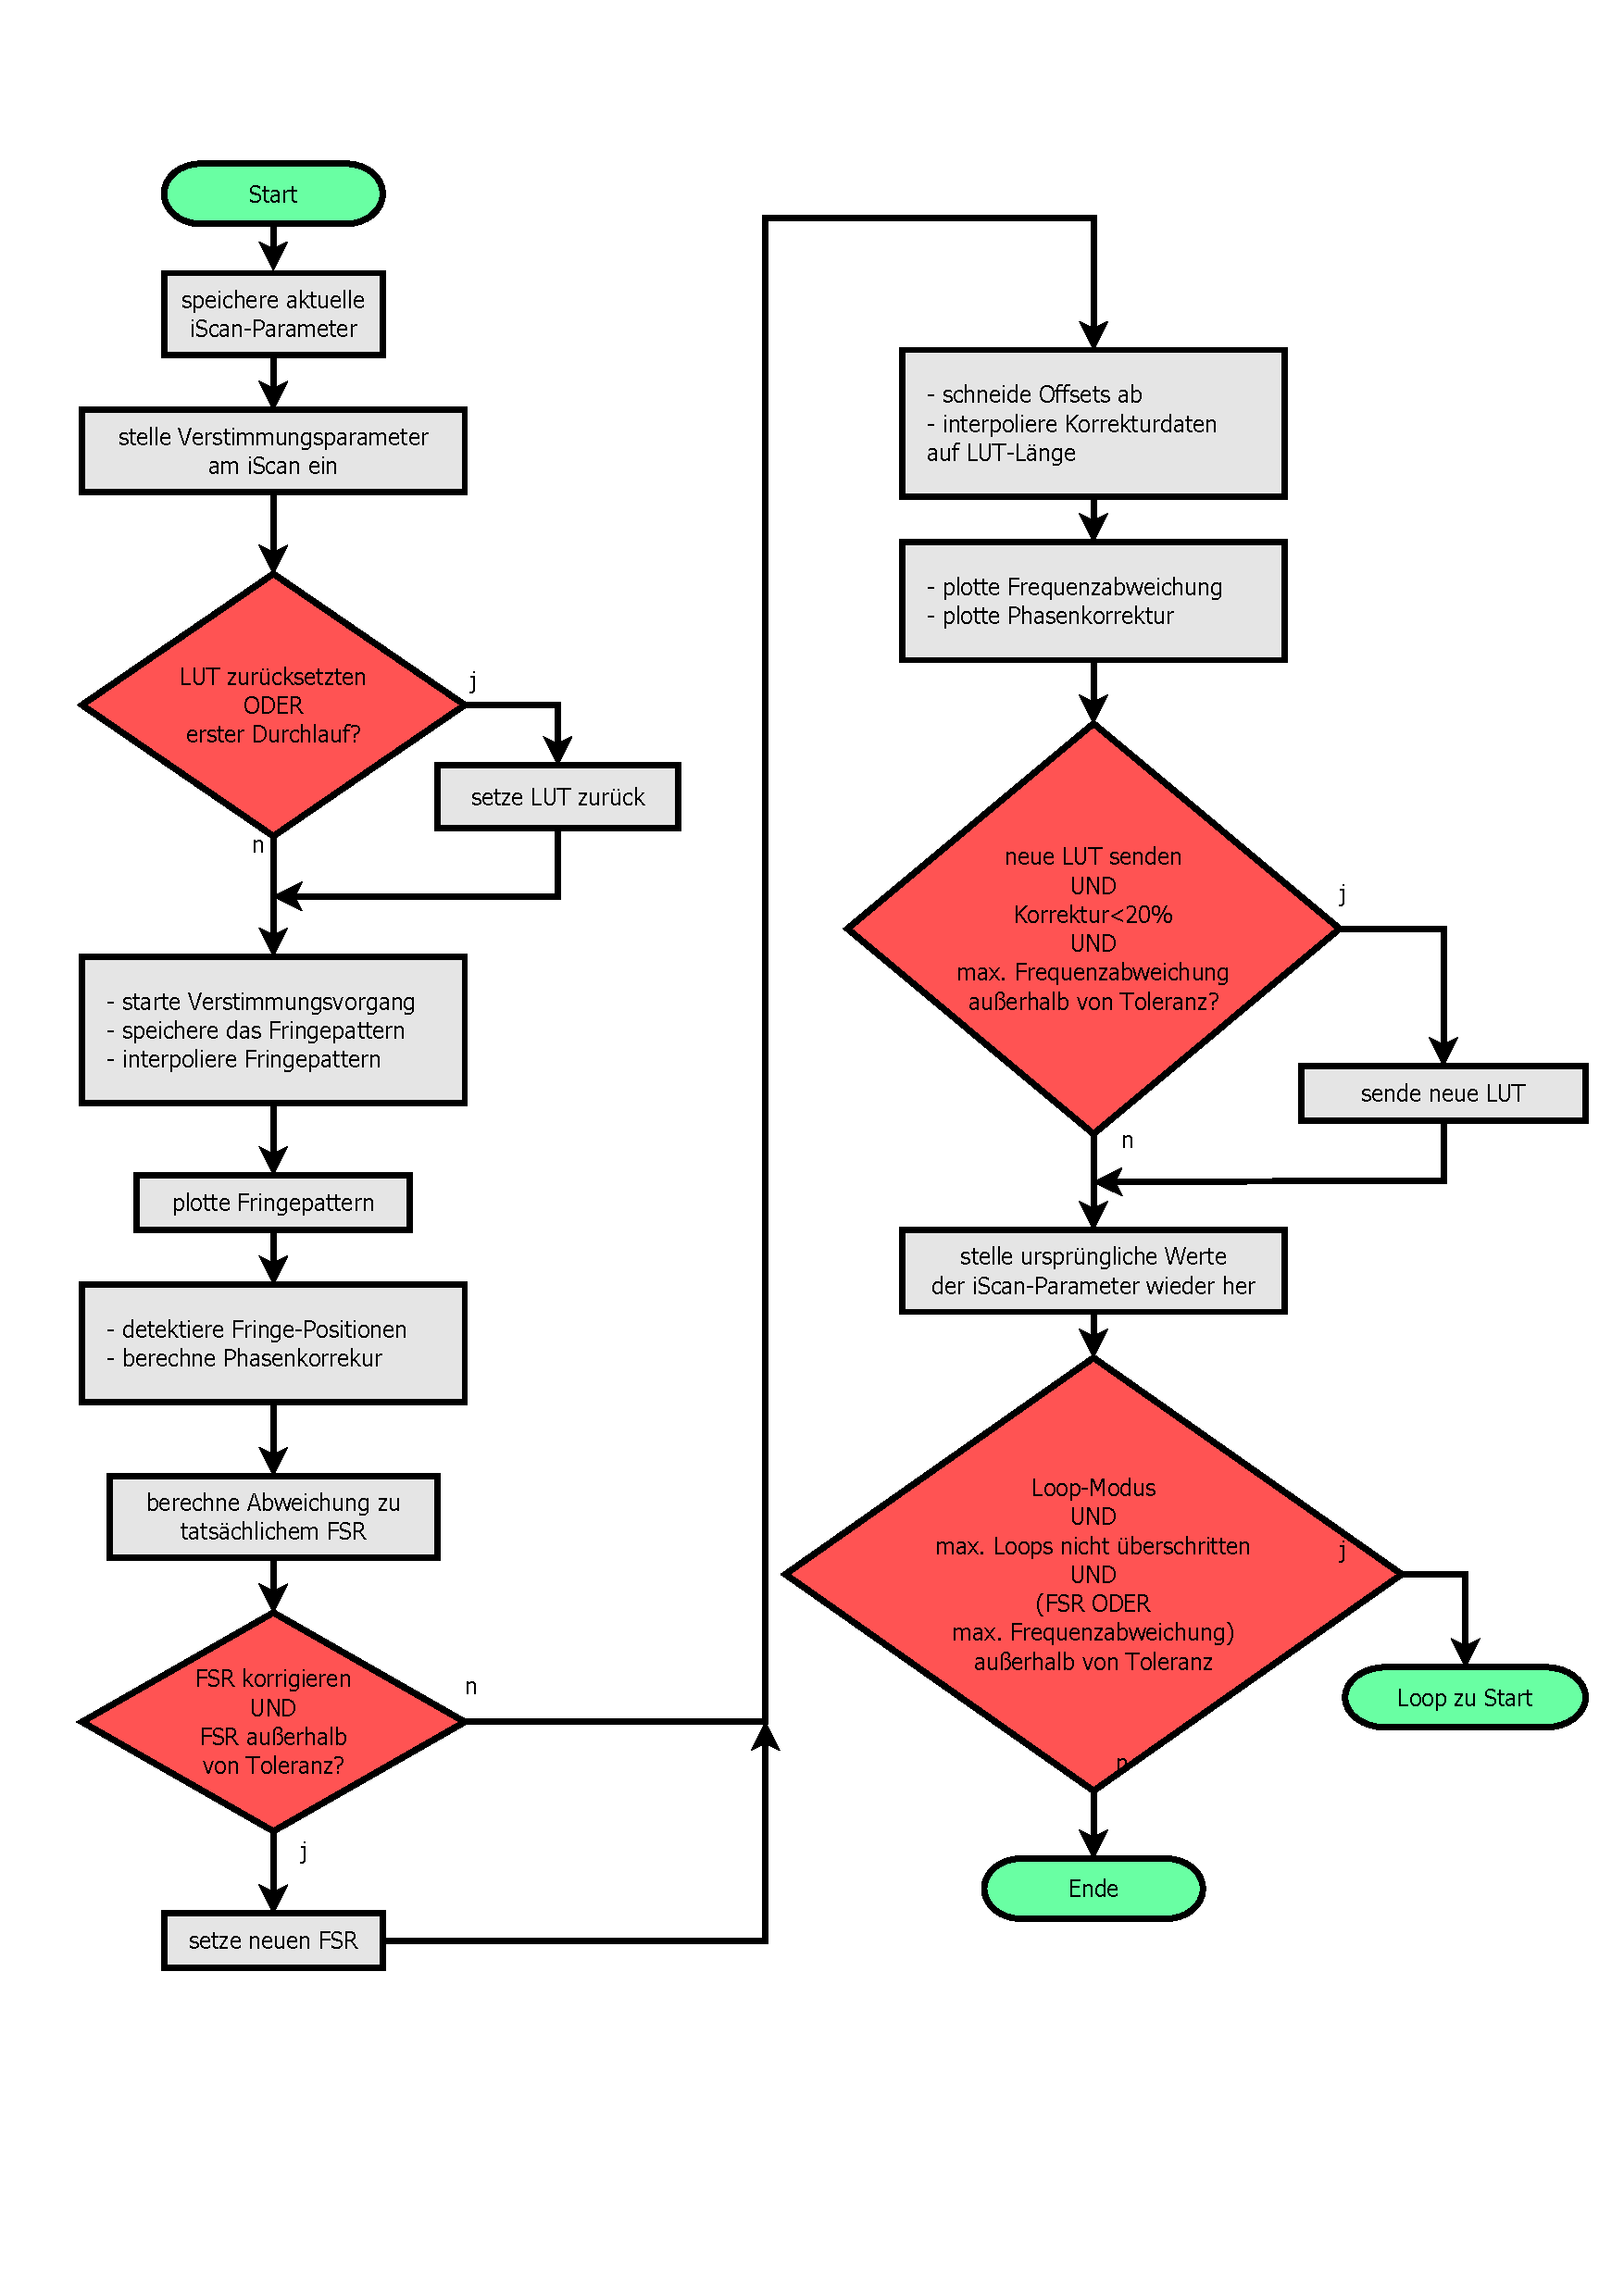
\includegraphics[width=\textwidth-0.5cm]{gfx/linearisierung_ablaufdiagramm}
	    }}
	\caption[Linearisierung der \textit{iScans} -
	Ablaufdiagramm]{Ablaufdiagramm der
	Linearisierung der \textit{iScans}}\label{fig:linearisierung_ablaufdiagramm}
\end{figure}
Zunächst werden alle relevanten aktuellen \textit{iScan}-Parameter
zwischengespeichert, damit sie am Ende der Routine wieder zurückgeschrieben
werden können. Über welchen Frequenzbereich das Fringepattern abgefahren wird,
legt Parameter \lstinline|FSR| fest.
Prozentual zu \lstinline|FSR| wird ein Offset berechnet, mit dem der abzufahrende Frequenzbereich erweitert wird, damit
Nichtlinearitäten am Anfang und am Ende des Bereichs abgeschnitten werden
können. Beim ersten Durchlauf der Linearisirungsroutine wird die LUT
zurückgesetzt. Das bedeutet, sie wird mit Werten $A_i$ und $B_i$ gefüllt, die
die äquidistante Punkte auf einem Kreis repräsentieren. Sind alle nötigen
Parameter gesetzt, beginnt das Abfahren der Frequenz linear zur LUT, wobei die
Messwerte des Fringepattern und die Frequenzwerte parallel in ein Array
gespeichert werden. Das Fringepattern wird auf der
Benutzeroberfläche angezeigt (siehe
\ref{fig:linearisierung_benutzeroberflaeche_fringepattern}).\par
\begin{figure}[h]
 	\centering
 	\fbox{\parbox{\dimexpr \linewidth - 2\fboxrule - 2\fboxsep}{
 	\centering
	    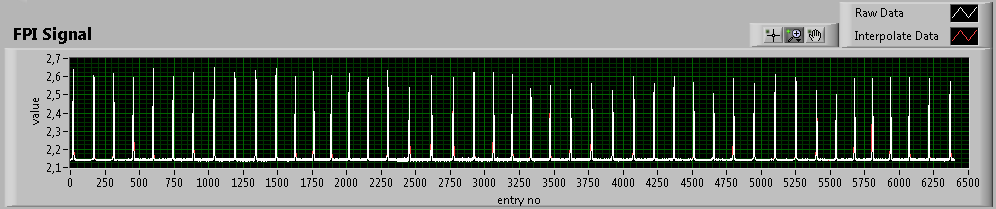
\includegraphics[width=\textwidth-0.5cm]{gfx/linearisierung_benutzeroberflaeche_fringepattern}
	    }}
	\caption[Benutzeroberfläche Linearisierung -
	Fringepattern]{Ausgabe des Fringepatterns und dessen Interpolation auf der
	Benutzeroberfläche.}\label{fig:linearisierung_benutzeroberflaeche_fringepattern}
\end{figure}
Vor der Weiterverarbeitung des Fringepattern wird dieses zur Glättung mehrfach
Interpoliert, damit es keine Probleme bei der Positionsbestimmung der Fringes
gibt. Das interpolierte Fringepattern wird nun in ein leider
geschütztes\footnote{Quelltext nicht offen} SubVI von \textit{TEM-Messtechnik}
gegeben, das die Fringepositionen detektiert, die Frequenzabstände der Fringes
untereinander analysiert und ein Array mit der aktuellen Phasenabweichung von
der Linearität ausgibt. Anschleißend wird das Array negiert, dessen Offsets
abgeschnitten und auf die Länge $N$ der LUT-Tabelle interpoliert, sodass sich
$N$ Phasenkorrekturwerte $\Delta\phi_i$ im Intervall
$[0,\text{\lstinline|FSR|}]$ ergeben. Die neuen LUT-Einträge
\begin{equation}\label{eq:LUT_korrektur_01}
	\begin{split}
		A_i&=-A\cdot\cos{\left(2\pi\frac{i}{N}+\Delta\phi_i\right)}\\
		&\text{und}\\
		B_i&=B\cdot\sin{\left(2\pi\frac{i}{N}+\Delta\phi_i\right)}\,.
	\end{split}
\end{equation}
werden durch modulieren einer Kreisquadratur mit der Phasenkorrektur
berechnet und in die LUT-Tabelle geschrieben. Ist die
maximale Frequenzabweichung nach der Korrektur nicht unter einem bestimmten Toleranzwert, wird die Routine ein weiteres Mal durchlaufen,
wobei die LUT eingangs nicht mehr zurückgesetzt wird. Stattdessen werden
die neuen Korrekturwerte über
\begin{equation}\label{eq:LUT_korrektur_02}
	\Delta\phi_i=\Delta\phi_{i,alt}-\Delta\phi_{i,akt}
\end{equation}
berechnet, wobei $\Delta\phi_{i,alt}$ die Korrekturwerte $\Delta\phi_i$
des vorherigen Durchlaufs und $\Delta\phi_{i,akt}$ die aktuellen Korrekturwerte
sind. Das Aufnehmen des Fringepattern und die Phasenkorrektur wiederholt sich so
lange bis, der Toleranzwert unterschritten wurde. Abbildung
\ref{fig:linearisierung_benutzeroberflaeche_phasenkorrektur} zeigt die Ausgabe der Phasenkorrektur auf der Benutzeroberfläche mit eingangs zurückgesetzter LUT.\par
\begin{figure}[h]
 	\centering
 	\fbox{\parbox{\dimexpr \linewidth - 2\fboxrule - 2\fboxsep}{
 	\centering
	    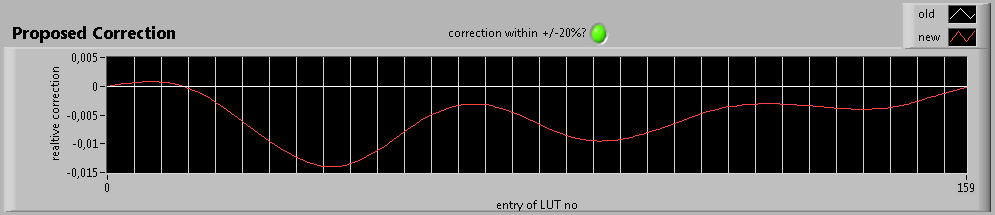
\includegraphics[width=\textwidth-0.5cm]{gfx/linearisierung_benutzeroberflaeche_phasenkorrektur}
	    }}
	\caption[Benutzeroberfläche Linearisierung -
	Phasenkorrektur]{Ausgabe der Phasenkorrektur nach erstmaligem Linearisieren auf
	der Benutzeroberfläche.}\label{fig:linearisierung_benutzeroberflaeche_phasenkorrektur}
\end{figure}
Neben der Linearität der \textit{iScans} kann auch die Korrektur des Parameters
\lstinline|FSR| bestimmt werden. Dazu betrachtet man zunächst die
Abweichung der \textit{iScan}-Skala zur tatsächlichen Frequenz. In
\ref{fig:linearisierung_benutzeroberflaeche_frequenz-abweichung} ist die
Ausgabe der Abweichung auf der Benutzeroberfläche dargestellt.
\begin{figure}[h]
 	\centering
 	\fbox{\parbox{\dimexpr \linewidth - 2\fboxrule - 2\fboxsep}{
 	\centering
	    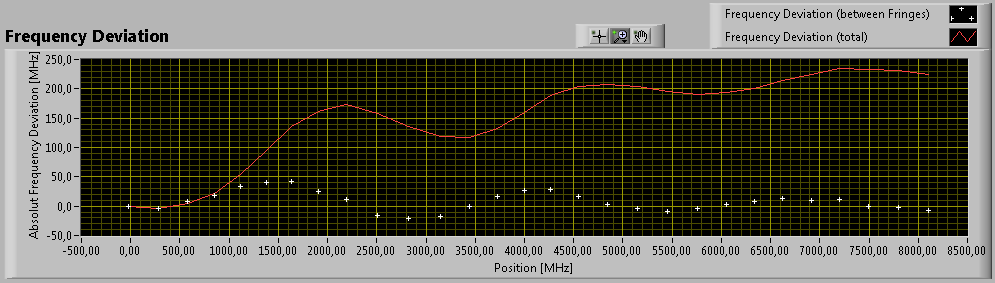
\includegraphics[width=\textwidth-0.5cm]{gfx/linearisierung_benutzeroberflaeche_frequenz-abweichung}
	    }}
	\caption[Benutzeroberfläche Linearisierung -
	Frequenzfehler]{Ausgabe	des Frequenzfehlers auf der
	Benutzeroberfläche.}\label{fig:linearisierung_benutzeroberflaeche_frequenz-abweichung}
\end{figure}
Die weißen Punkte stellen die Abweichung der einzelnen Fringeabstände zum FSR
des FPIs dar. Die rote Kurve beschreibt den totale Fehler des \textit{iScans} relativ zur
Startfrequenz. Endet die Kurve bei $\nu=\text{\lstinline|FSR|}$ ohne Fehler,
kann man davon ausgehen, dass der Parameter \lstinline|FSR| auch den
tatsächlichen FSR des \textit{iScans} repräsentiert. Ist der Fehler bei
$\nu=\text{\lstinline|FSR|}$ allerdings $>0$ bzw. $<0$, so ist
der Paramater \lstinline|FSR| zu klein bzw. zu groß gewählt und muss ensprechend
nachkorrigiert werden.\par
Problem bei der Berechnung der Abweichung zum wahren Wert des FSRs ist, dass nur
diskrete Messpunkte im Frequenzabstand von einem FPI-FSR, also ca. $300\,MHz$
vorliegen. Eine Möglichkeit ist, nach erfolgreicher Linearisierung einen
linearer Fit der totalen Frequenzabweichung zu machen. Die Differenz der Offsets bei
$\nu=0$ und $\nu=\text{\lstinline|FSR|}$ ergibt dann den Korrekturwert. Eine
genauere und linearisierungsunabhängige Methode, die hier implementiert wurde,
soll im Folgenden kurz erleutert werden.\par

